% !TEX root = /home/fred-olav/afgv/src/preamble.tex
\input preamble.tex
\centerline{\bf Juleprøve 2020 - Automatiseringsystemer}  \bigskip

Kompetansemål:
\begin{itemize}[noitemsep]

	\item Prøven dekker alle kompetansemål i automatiseirngsfaget fra VG1 til VG3 auto.  
\end{itemize}

Alle ark som leveres inn skal ha elevens navn. \\ 

Oppgave 1 leveres på papir til Sigmund. \\
Oppgave 2 leveres på papir til Geir Atle \\
Oppgave 3 og 4 skal leveres på papir til Jon\\
Oppgave 1-8 skal leveres på papir til Fred-Olav. \\
Oppgave 9 skal gjøres i  på PC og det skal levers en PC|Schematic file og en codesys fil. Disse sendes på mail til fred-olav.mosdal@skole.rogfk.no med emne Juleprøve

\bigskip 
\hrule
\bigskip 
\hrule
\vfil \eject
ss
\eject
Oppgave 1

a) Hva er forskjellen på en digital ultralydgiver, og en analog ultralydgiver?


\begin{tikzpicture}
	\draw[step=0.5cm,gray!20,very thin]  grid (16,4) ;
\end{tikzpicture}
b) De to bryterende på skjemaet skal kobles til en normalt lukket sløyfe til inngang Ix.0. 

$$\includegraphics[width=12.5cm]{i04811x01.eps}$$
c) På ett postsorteringsanlegg skal pakkene skilles etter størrelse, kom med forslag om hvilke givere du kunne brukt og hvordan?


\begin{tikzpicture}
	\draw[step=0.5cm,gray!20,very thin]  grid (16,6) ;
\end{tikzpicture}
\filbreak
d) Det er behov for å vite posisjonene på aksene Z,Y og X på 3D printeren. Hva kan brukes for å måle posisjonenene, og er det forskjellige metoder for noen som tåler strømtap, og for å få bedre nøyaktighet

$$\includegraphics[width=10cm]{../output/3dprinter.png}$$


\begin{tikzpicture}
	\draw[step=0.5cm,gray!20,very thin]  grid (16,8) ;
\end{tikzpicture}
%\vfil
Oppgave 2


a) Før på hva det er: \\ 

$$\includegraphics[width=15.5cm]{../output/motor.png}$$

\begin{enumerate}
	\item 
	\item 
	\item 
	\item 
	\item 
	\item 
	\item 
\end{enumerate}

\filbreak
b) Merkeskilt for en ny (brukt) elektrisk motor som skal brukes: \\

\begin{center}
\begin{tabular}{ | m{3cm} | m{3cm} | } 
\hline
\multicolumn{2}{|c|}{Merkeskilt} \\
\hline
Motor 3~ 50Hz	& IEC34-6-IC01 \\ 
\hline
4 kW & 2880 r/m \\
\hline
Y 400V 8.0A & $\Delta$230V 13.8A \\
\hline
& cos$\varphi$ 0.8 \\
\hline
& IP 54 \\
\hline
\end{tabular}
\end{center}

\begin {itemize}

\item Hva blir tilført effekt? 
\\\\

\begin{tikzpicture}
	\draw[step=0.5cm,gray!20,very thin]  grid (15,4) ;
\end{tikzpicture}
\item Hvor stor blir virkningsgraden $\eta$  ?
\\\\

\begin{tikzpicture}
	\draw[step=0.5cm,gray!20,very thin]  grid (15,4) ;
\end{tikzpicture}
\item Synkront omdreiningstall for motoren?
\\\\

\begin{tikzpicture}
	\draw[step=0.5cm,gray!20,very thin]  grid (15,4) ;
\end{tikzpicture}
\item Sakkingen blir da i prosent?
\\\\

\begin{tikzpicture}
	\draw[step=0.5cm,gray!20,very thin]  grid (15,4) ;
\end{tikzpicture}
\item Antall polpar? 
\\\\

\begin{tikzpicture}
	\draw[step=0.5cm,gray!20,very thin]  grid (15,4) ;
\end{tikzpicture}
\end {itemize}
\filbreak
c) Motoren er en ny (brukt) og må måle verifiseres før tilkobling. Hva og hvor vil du måle?\\

\begin{tikzpicture}
	\draw[step=0.5cm,gray!20,very thin]  grid (16,14) ;
\end{tikzpicture}
d) Motoren skal kobles til et IT- nett, tegn klemmebrettet og vis hvor laskene må plasseres og hvor L1, L2 og L3 skal tilkobles. \\

\vfil
\vfil
Oppgave 3


a) Kva er trykk og kraft og kva eining har dei? (formel) 
\\

\begin{tikzpicture}
	\draw[step=0.5cm,gray!20,very thin]  grid (15,4) ;
\end{tikzpicture}
\\
b) Kva er største måleomfang, minste måleomfang og kalibrert måleomfang til ein transmitter? 
\\

\begin{tikzpicture}
	\draw[step=0.5cm,gray!20,very thin]  grid (15,4) ;
\end{tikzpicture}
\\
c) Kva er hydrostatisk trykk? 
\\\\

\begin{tikzpicture}
	\draw[step=0.5cm,gray!20,very thin]  grid (15,4) ;
\end{tikzpicture}
\\
d) Kva er dødbandet når vi målar nivået med for eks. ein ultralydmålar? 
\\\\

\begin{tikzpicture}
	\draw[step=0.5cm,gray!20,very thin]  grid (15,4) ;
\end{tikzpicture}
\\
e) Kva er dette, og korleis verkar det?	 
\\\\
$$\includegraphics[width=8cm]{../output/jon1.png}$$

\begin{tikzpicture}
	\draw[step=0.5cm,gray!20,very thin]  grid (15,4) ;
\end{tikzpicture}
\\
\eject
f) Nemn minst 2 trykkmålarprinsipp som blir bruka i trykktransmittere, og forklår korleis dei verkar? 
\\\\

\begin{tikzpicture}
	\draw[step=0.5cm,gray!20,very thin]  grid (15,4) ;
\end{tikzpicture}
\\
g) Forklår korleis vi monterer trykktransmittere inn på ei røyrlinje som enten fører veske, damp eller gass. 
\\\\

\begin{tikzpicture}
	\draw[step=0.5cm,gray!20,very thin]  grid (15,10) ;
\end{tikzpicture}
\\
\eject
h) I mange av trykkmåle instrumenta skal vi måle svært små forskjellege storleikar (Ampere, volt, ohm). Kvifor brukar vi Wheatstone’s målebru i denne samanheng? Teikn skisse og forklår. 
\\\\

\begin{tikzpicture}
	\draw[step=0.5cm,gray!20,very thin]  grid (15,10) ;
\end{tikzpicture}
\\
j) Ein oljetank med volum på 750 m3. Diameteren på tanken er 10m. Finn trykket i botnen når? 
\\\\
\begin{enumerate}


 \item Tanken er full
 \item Tanken er 75% full
 \item Tanken er 30% full

\end{enumerate}

Densiteten til olja i tanken er 0,82 · 103 kg/m3.
	 \\

\begin{tikzpicture}
	\draw[step=0.5cm,gray!20,very thin]  grid (15,8) ;
\end{tikzpicture}
Oppgave 4

a) Kva er eit termoelement? Teikn skisse og forklår korleis det verkar. Kva temperaturområde kan vi måle med eit termoelement?
\\

\begin{tikzpicture}
	\draw[step=0.5cm,gray!20,very thin]  grid (15,10) ;
\end{tikzpicture}
\\
\eject
b) Forklar korleis eit pt-100 element er oppbygd og korleis det verkar. Teikn skisser og forklar korleis det vert kopla til ein måleomformar. Kvifor brukar vi helst tre-leder kopling mellom pt-100 elementet og måleomformaren.
\\

\begin{tikzpicture}
	\draw[step=0.5cm,gray!20,very thin]  grid (15,10) ;
\end{tikzpicture}
\\
c) Forklar uttrykka i måleteknikken: 
\begin{enumerate}
\item Tidskonstanten
\item Øvre målegrense
\item Nedre målegrense
\item Måle område
\end{enumerate}


\begin{tikzpicture}
	\draw[step=0.5cm,gray!20,very thin]  grid (15,8) ;
\end{tikzpicture}
\\

d) Nemn minst 5 forskjellege måleprinsipp for nivå i ein behaldar, og forklar måleprinsippet med ultralyd. Kva fordel er der med radarprinsippet i staden for ultralyd? 
\\

\begin{tikzpicture}
	\draw[step=0.5cm,gray!20,very thin]  grid (15,10) ;
\end{tikzpicture}
\\
e) Teikn skisse av ei veiecelle basera på strekklapp prinsippet og forklår korleis den verkar. Når er det mest aktuelt å bruka veieceller til nivåmåling?
\\

\begin{tikzpicture}
	\draw[step=0.5cm,gray!20,very thin]  grid (15,8) ;
\end{tikzpicture}
\\
f) Teikn ei prinsippskisse for ei hydraulisk veiecelle. 
\\

\begin{tikzpicture}
	\draw[step=0.5cm,gray!20,very thin]  grid (15,8) ;
\end{tikzpicture}
\eject 
g) Nemn nokre måleomformarar for nivå med av/på utgang. Kva kan vi bruke dei til?
\\

\begin{tikzpicture}
	\draw[step=0.5cm,gray!20,very thin]  grid (15,8) ;
\end{tikzpicture}
\\
\vfil
\eject
Oppgave 5 \\


a) Tegn inn ledninger sånn at det lages en paralellkrets der strømmen følger pilene på
hver motstand.
\vfil
$$
\includegraphics[width=8cm]{i04814x01.eps}$$

\vfil
b) Tegn inn ledninger sånn av det lages en seriekrets der strømmen følger pilene på hver motstand.
$$
\includegraphics[width=8cm]{i04814x02.eps}$$

\filbreak
c) Tegn in ledninger slik at de to parallelle motstandene kommer i serie med den enkle motstanden. Koble så kretsen til batteriet.

$$\includegraphics[width=15cm]{i04814x03.eps}$$

d) Tegn inn ledninger sånn at NO brytere vil aktivere releet når den trykkes inn. Releet skal igjen gi strøm til lampen slik at den lyser.

$$\includegraphics[width=15cm]{i04814x04.eps}$$

\filbreak
e) Tegn inn legninger som viser hvordan den kontaktløse radar nivåmåleren skal kobles for og sende prosessveriden til inngang 1 på regulatoren. Du kan anta at strømsløyfen på nivåmåleren er av 4 leder type.
$$\includegraphics[width=15cm]{i04814x05.eps}$$
\eject
Oppgave 6\\


a) En SMART DP-celle er tatt ut av drift og tatt med for benkkalibrering. En automatikker kobler til et presisjons trykkmanometer og en luftkilde til High inngangen på DP-cellen, mens han måler strømutgangen med et multimeter. 

$$\includegraphics[width=15.5cm]{i04815x01.eps}$$

Regn ut avviket i \% av måleområde for {\it sensor trim} og avviket i  \% av måleområde for {\it utgangstrim}.  Forklar hvorfor en må ha en HART kommunikator for å kunne regne disse avvikene sepparat. 


b) Fyll ut kalibreringstabellen for dette strømningsmålesystemet. Systemet består av en måleblende, DP-celle, kvadratrotuttrekker og indikator. Du kan anta følgende måleområder:

Husk:\\
$$Q \propto \sqrt{\Delta P }$$

$$\includegraphics[width=15.5cm]{i00048x01.eps}$$

\begin{itemize}
\item{} FE: 0-50 L/s, 0-100 cmWC  $\Delta$P
\item{} FT: 0-100 cmWC inn, 4-20 mA ut (linear)
\item{} FY: 4-20 mA inn and ut (kvadratrot)
\item{} FI: 4-20 mA inn, 0-50 L/s avlesning
\end{itemize}

% No blank lines allowed between lines of an \halign structure!
% I use comments (%) instead, so that TeX doesn't choke.

$$\vbox{\offinterlineskip
\halign{\strut
\vrule \quad\hfil # \ \hfil & 
\vrule \quad\hfil # \ \hfil & 
\vrule \quad\hfil # \ \hfil & 
\vrule \quad\hfil # \ \hfil & 
\vrule \quad\hfil # \ \hfil & 
\vrule \quad\hfil # \ \hfil \vrule \cr
\noalign{\hrule}
%
% First row
Flow rate & Percent of & Orifice $\Delta$P & FT output & FY output & FI indication \cr
%
% Another row
(L/s) & max. flow (\%) & (cmWC) & signal (mA) & signal (mA) & (L/s) \cr
%
\noalign{\hrule}
%
% Another row
0 & 0 &   &   &   & 0 \cr
%
\noalign{\hrule}
%
% Another row
  & 10 &   &   &   &  \cr
%
\noalign{\hrule}
%
% Another row
  & 25 &   &   &   &  \cr
%
\noalign{\hrule}
%
% Another row
25 & 50 &   &   &   & 25 \cr
%
\noalign{\hrule}
%
% Another row
  & 75 &   &   &   &  \cr
%
\noalign{\hrule}
%
% Another row
  & 90 &   &   &   &  \cr
%
\noalign{\hrule}
%
% Another row
50 & 100 &   &   &   & 50 \cr
%
\noalign{\hrule}
} % End of \halign 
}$$ % End of \vbox

\vfil
Oppgave 7

a )Hva menes med følgende begreper:

\begin{itemize}
\item Regulator
\\\\

\begin{tikzpicture}
	\draw[step=0.5cm,gray!20,very thin]  grid (15,2) ;
\end{tikzpicture}
\item ProsessVerdi PV 
\\\\

\begin{tikzpicture}
	\draw[step=0.5cm,gray!20,very thin]  grid (15,2) ;
\end{tikzpicture}
\item Prosess
\\\\

\begin{tikzpicture}
	\draw[step=0.5cm,gray!20,very thin]  grid (15,2) ;
\end{tikzpicture}
\item Pådragsorgan
\\\\

\begin{tikzpicture}
	\draw[step=0.5cm,gray!20,very thin]  grid (15,2) ;
\end{tikzpicture}
%\item Forstyrrelse 
\item Regulatorens modus (auto/manuell) 
\\\\

\begin{tikzpicture}
	\draw[step=0.5cm,gray!20,very thin]  grid (15,2) ;
\end{tikzpicture}
\end{itemize}



\vfil
\eject

b) Tegn blokkskjema for en reguleringssløyfe. 

\vfil

\eject

c) Tegn grafen for utgangen  for en reverserende regulator med $K_p=3$ og BIAS=50\%. 
%Qualitatively graph the response of a proportional-plus-derivative controller over time to the following changes in process variable:

$$\includegraphics[width=15.5cm]{i04816x01.eps}$$


\begin{tikzpicture}
	\draw[step=0.5cm,gray!20,very thin]  grid (16,9) ;
\end{tikzpicture}
\eject
d) Forklar hvordan dette \textit{kaskadekoblede} temperaturreguleringssystemet virker.

$$\includegraphics[width=15.5cm]{i01690x01.eps}$$

Finn ut hvilken retning styresignalet må ha på hver av regulatorene. Du kan anta direkte virkende ytransmittere og air-to-open ventil. Merk skjemaet med pil opp og ned symboler for å finne ut hvilken virkning PV og SP har på regulatoren. \\


\begin{tikzpicture}
	\draw[step=0.5cm,gray!20,very thin]  grid (16,9) ;
\end{tikzpicture}
Oppgave 8

Hydrogenreforming er en prosess der spesielle brennkammer brukes for å lage rent hydrogen fra hydrocarboner. Metan gass (CH$_{4}$) blandes med damp (H$_{2}$O) under høy  temperatur. Da dannes H$_{2}$) og karbonmonodksyd (CO), som i gjen omformes til CO$_{2}$. Denne reaksjonen er endotermisk, som vil si at den krever energi. Denne energien tilføres i et brennkammer. 

$$\includegraphics[width=15.5cm]{i02504x01.eps}$$

Mengden hydrokarboner som tilføres prosessen påvirker i høy grad temperaturen inne i forbrenningskammeret, noe som gjør det utfordrende å holde temperaturen på settpunktet. Skisser en løsning på dette temperaturstabilitetsproblemet ved å bruke forkover koblet regulering. 
%The rate of hydrocarbon feed greatly ``loads'' the control of temperature inside the reaction furnace, making it more challenging to maintain setpoint temperature as the feed rate varies.  Design a solution for this temperature-stability problem using a {\it feedforward} control strategy, explaining the reasoning behind your solution.



b) En prosess gir følgende graf ved et sprang i pådraget

$$\includegraphics[width=15.5cm]{i01662x01.eps}$$

Hvilken type prosess er dette?


c) En prosess gir følgende graf ved et sprang i pådraget

$$\includegraphics[width=15.5cm]{i01663x01.eps}$$

Hvilken type prosess er dette?

d) Regn ut følgende basert på at transmitteren er kalibrert for et måleområde fra 50mbar til 400mbar. Transmitteren har et utgangssignal på 4-20mA \\
Vis alle utregninger. \\
$$\includegraphics[width=15.5cm]{i04815x02.eps}$$



\begin{itemize}
\item{} $I$ = \underbar{\hskip 50pt} mA
\vskip 10pt
\item{} $U_{C}$ = \underbar{\hskip 50pt} V 
\vskip 10pt
\item{} $U_{BC}$ = \underbar{\hskip 50pt} V 
\vskip 10pt
\item{} $U_{B}$ = \underbar{\hskip 50pt} V 
\end{itemize}

\filbreak
Oppgave 9

Se medfølgende  P\&ID til denne skal du:

\begin{enumerate}
	\item Plukke ut IO moduler i wago sin 750 serie som kan ta imot signalene fra P \& ID-en. 
\item Tegne koblingsskjema for alle signalene i PC|Schematic
\item Opprette et prosjekt i Codesys og vise hvordan modulene legges inn der for så å koble signalene mot en PID regulator. 
\item Lage en HMI som kan brukes til å optimalisere prosessen. (det forventes bruk av graf.)
\end{enumerate}


$$\includegraphics[width=15.5cm]{i04819x01.pdf}$$


\end {document}
